\chapter{Simon's Algorithm}
This problem is another one of the completely artificial problems, but now the advantage of quantum over probabilistic approaches is quite significant: a linear number of queries will be needed by the quantum algorithm, whereas an exponential number will be needed for any classical probabilistic algorithm. Although the problem is artificial, it is surprisingly close to a very natural and important real-world problem, as we will see. Also, the quantum algorithm for this problem introduces some powerful techniques in a simple form. It is interesting for the following two reasons:

\begin{enumerate}
    \item It improves on the progression of black-box problems where quantum algorithms outperform classical algorithms. The quantum algorithm requires exponentially fewer queries than even probabilistic classical algorithms that can err with constant probability, say $\frac{1}{4}$.
    
    \item The quantum algorithm for Simon's problem introduces a technique that transcends the black-box model. When viewed in the right way, the ideas introduced in Simon's algorithm lead naturally to Shor's algorithm for the discrete logarithm problem — which is not a black-box model problem! Shor discovered his algorithms (for discrete logarithms and factoring) soon after seeing Simon's algorithm, and in his paper, he acknowledges that he was inspired by Simon's algorithm.
\end{enumerate}

\section{The Problem Definition}

\begin{definition}
    Given a function $f:\{0,1\}^n \rightarrow \{0,1\}^n$ which takes $n$ input bits and returns $n$ output bits (for a positive integer $n$), the function is a \textit{two-to-one} function. This means that for every point in the range, there are exactly two pre-images. In other words, for every value that the function attains, there are exactly two points $a$ and $b$ in the domain such that both map to that value.

    The function satisfies $f(a) = f(a \oplus s)$ for some non-zero bit string $s \in \{0,1\}^n$. We are required to find $s$. Similar to the Deutsch-Jozsa problem, the function $f$ is promised to obey a certain property, although this property is slightly more complicated than before.

    \[
    f(a) = f(b) \iff a \oplus b \in \{0^n, s\}
    \]

    Here, $\oplus$ denotes the bitwise sum modulo 2 (bitwise XOR). That is, you take the XOR of the first bit of $a$ with the first bit of $b$, then the XOR of the second bit of $a$ with the second bit of $b$, and so on. For example, $1101 \oplus 0111 = 1010$ and $01 \oplus 01 = 00$.

    A pair of points $(a, b)$ such that $x \neq y$ and $f(a) = f(b)$ is called a \textit{colliding pair}. Note that for every colliding pair $(a, b)$, we have $a \oplus b = s$.
\end{definition}


\begin{example}
    Consider the function $f:\{0,1\}^3 \rightarrow \{0,1\}^3$ for $n = 3$, and let $s = 111$. Since the function is a two-to-one function (i.e., it produces the same output for two distinct inputs such that $f(x) = f(x \oplus s)$), we have:
    \begin{align*}
        f(000) &= f(000 \oplus 111) = f(111); \quad 
        f(001) = f(001 \oplus 111) = f(110); \\ 
        f(010) &= f(010 \oplus 111) = f(101); \quad 
        f(011) = f(011 \oplus 111) = f(100); \\
        f(100) &= f(100 \oplus 111) = f(011); \quad 
        f(101) = f(101 \oplus 111) = f(010); \\
        f(110) &= f(110 \oplus 111) = f(001); \quad 
        f(111) = f(111 \oplus 111) = f(000).
    \end{align*}
    Thus, we have:
    \begin{align*}
        f(000) &= f(111), \\
        f(001) &= f(110), \\
        f(010) &= f(101), \\
        f(011) &= f(100).
    \end{align*}

    Consider the following function output in tabular form:
    \begin{table}[H]
        \centering
        \begin{tabular}{|c|c|}
            \hline
            Input & Output \\
            \hline
            000 & 111 \\
            001 & 000 \\
            010 & 110 \\
            011 & 010 \\
            100 & 010 \\
            101 & 110 \\
            110 & 000 \\
            111 & 111 \\
            \hline
        \end{tabular}
        \caption{Example of Simon's algorithm}
        \label{tab:exsimon}
    \end{table}

    It can be clearly seen that the above function is valid, as it satisfies the constraints of being a two-to-one function. We can also see from Table~\ref{tab:exsimon} that the function is periodic with period $s = 111$, thus following Simon's promise.

    Hence, this is a valid example function for Simon's algorithm.

    Now, given that the function is two-to-one, we are required to find $s$. Note that if you take any colliding pair $(x, y)$, then $x \oplus y$ is always the same 3-bit string. For example, take $001$ and $110$, which is a colliding pair since $x = 001 \neq y = 110$ and $f(x) = f(001) = f(110) = 000$. Then, $x \oplus y = 001 \oplus 110 = s = 111$.

    Note that for an arbitrary two-to-one function, the bitwise XORs can be different for different colliding pairs. So, the two-to-one functions that satisfy the Simon property are special: their bitwise XORs are always the same.
\end{example}


\section{The Classical Solution}

\textbf{On a Classical Computer:} One way to solve this is to find a colliding pair. But notice that any two distinct $n$-bit strings could be a colliding pair for some $s$. So, if we make a query at some point $a$, we learn the value of $f(a)$, but we have no idea for which $b \neq a$ we will get a colliding pair.

In order to determine the period of the function, we need to query the function $2^{n-1} + 1$ times. This is because the total number of possible inputs is $2^n$, and since the function is two-to-one with a period $s$, it produces the same output for exactly half of the inputs. Thus, in the worst-case scenario, we must query the function $2^{n-1} + 1$ times to guarantee discovering a collision and hence determine the period.

Once we have a colliding pair, it's easy to find $s$ by taking the bitwise XOR of the pair. Therefore, the time complexity of the classical algorithm is $\mathcal{O}(2^n)$, i.e., exponential time complexity.

The best classical approach is to use randomized algorithms with a probabilistic strategy. For example, if we have a budget of $m$ queries, we query $f$ at $m$ random points in $\{0,1\}^n$ and then check if there's a collision among them. If any two inputs form a colliding pair, then their bitwise XOR is the answer $s$. If there are no collisions, then the algorithm is out of luck; in that case, it fails to find $s$.

How large should $m$ be so that the probability of a collision is at least $3/4$? Since there are $2^n$ points in the domain, and each pair of queries will collide with probability $\frac{1}{2^n}$, and there are roughly $m^2$ such pairs, the expected number of collisions is roughly $m^2 \cdot \frac{1}{2^n}$. Setting $m = \sqrt{2^n}$ suffices to make this expectation constant. In this case, the expected running time becomes $\mathcal{O}(2^{n/2})$, which is still exponential.

You may recognize in this analysis the so-called “birthday paradox,” where you consider the probability that there are two people in a group (say, 23 people) who share the same birthday. It turns out to be about 50\%, assuming birthdays are uniformly distributed. 

Note that once we know two inputs (say, $a$ and $b$) with the same output, then we can use $a \oplus b = s$ to find $s$, because:
\[
b = a \oplus s \implies a \oplus b = a \oplus (a \oplus s) = (a \oplus a) \oplus s = 0 \oplus s = s.
\]


\subsection{Classical Lower Bound}
\begin{theorem}
    Any classical algorithm that solves the Simon's problem with worst-case success probability at least $\frac{3}{4}$ must make $\Omega(\sqrt{2^n})$ queries.
\end{theorem}
We cannot deduce this simply based in the fact that this is the best algorithm that we could come up with. How can we be sure that there isn't some clever trick that we haven't discovered?. Also, notice that $f$ is not an arbitrary two-to-one function. It is a two-to-one function with Simon property, which is a very special structure. So it's conceivable that a classical algorithm can somehow take advantage of that structure to find a collision in an unusual way.

The proof to the theorem is not as trivial and requires proof. Thus, now we shall begin with proof to this theorem.
\begin{proof}
    This proof uses some standard techniques that arise in computational complexity, however, this account assumes no prior background in the area.

    The first part of the proof is to ``play the adversary" by coming up with a way of generating an instance of $f$ that will be hard for any algorithm. Note that picking some fixed $f$ will not work very well. A fixed $f$ has a fixed $r$ associated with it and the first two queries of the algorithm could be $0^n$ and $r$, which would reveal $r$ to the algorithm after only two queries. rather, we shall randomly generate instances of $f$. First, we pick $r$ at random, uniformly from $\{0,1\}^n -0^n$. Picking $r$ does not fully specify $f$ but it partitions $\{0,1\}^n$ into $2^{n-1}$ colliding pairs of the form $\{x,x\oplus r\}$ in the lexicographic order. Let T be the set of all such representatives: $T=\{s:s=\min \{x,x\oplus r\} \text{for some } x \in \{0,1\}^n$ The we can define $f$ in terms of a random one-to-one function $\phi:T\rightarrow \{0,1\}^n$ uniformly over all the $2^n(2^n-1)(2^n-2)\ldots(2^n-2^{n-1}+1)$ possibilities. The definition of $f$ can then be taken as
    \[
    f(x) = \begin{cases} \phi(x) & \text{if } x \in T \\ 
    \phi(x \oplus r) &\text{if } x \notin T \end{cases}
    \]
    We shall prove that no classical probabilistic algorithm can succeed with probability $\frac{3}{4}$ on such instances unless it makes a very large number of queries.

    The next part of the proof is to show that, with respect to the above distribution among inputs, we need only consider deterministic algorithms (by which we means ones that make no probabilistic choices). The idea is that any probabilistic algorithm is just a probability distribution over all the deterministic algorithms, so its success probability $p$ is the average of the success probabilities of all the deterministic algorithms (where the average is weighted by the probabilities). At least one deterministic algorithm must have success probability $\geq p$ (otherwise the average would be less than $p$). Therefore (because we have a fixed probability distribution of the input instances), we need only consider deterministic algorithms.

    Next, consider some deterministic algorithm and the first query that it makes: $(x_1,y_1) \in \{0,1\}^n \times \{0,1\}^n$, where $x_1$ is the input to the query and $y_1$ is the output of the query. The result of this will just be a uniformly random element of $\{0,1\}^n$, independent of $r$. Therefore the first query by itself contains absolutely no information about $r$.

    Now consider the second query $(x_2,y_2)$ (without the loss of generality, we can assume that the inputs to all queries are different; otherwise the redundant queries could be eliminated from the algorithm). There are two possibilities: $x_1 \oplus x_2 =r$ (collision) or $x_1\oplus x_2 \neq r$ (no collision). But the first case arises with probability only $\frac{1}{2^n-1}$. With probability $1-\frac{1}{2^n-1}$, we are in the second case, and all the algorithm deduces about $r$ is that $r\neq x_1\oplus x_2$ (it has ruled out just one possibility among $2^n-1$).

    We continue our analysis of the process by induction on the number of queries. Suppose that $k-1$ queries, $(x_1,y_1),\ldots,(x_{k-1},y_{k-1})$ have been made without any collisions so far. (No collision so far means that, for all $1\leq i<j\leq k-1, y_i\neq y_j$). Then all that has been deduced about $r$ is that it is not $x_i \oplus x_j$ for all $1\leq i<j\leq k-1$. In other words, up to $(k-1)(k-2)/2$ possibilities of $r$ have been eliminated. When the next query $(x_k,y_k)$ is made, the number of potential collisions arising from it are at most $k-1$ (there are $k-1$ previously made queries to collide with). Therefore the probability of collision at query $k$ is at most
    \[
    \frac{k-1}{2^n-1-(k-1)(k-2)/2} \leq \frac{2k}{2^{n+1}-k^2}
    \]
    Since the collision probability bound in the above equation holds for all $k$, the probability of a collision occurring somewhere among $m$ queries is at most the sum of the right side of equation with $k$ varying from $1$ to $m$:
    \[
    \sum_{k=1}^m \frac{2k}{2^{n+1}-k^2} \leq \sum_{k=1}^m \frac{2m}{2^{n+1}-m^2} \leq \frac{2m^2}{2^{n+1}-m^2}
    \]
    If this quantity is to be at least $\frac{3}{4}$ then
    \[
    \frac{2m^2}{2^{n+1}-k^2} \geq \frac{3}{4}
    \]
    When we solve form in the above inequality, we get,
    \[
    m\geq \sqrt{\frac{6}{11}2^n}
    \]
    which gives the desired bound.

    Actually, there is a slight technicality remaining. We have shown that $\sqrt{(6/11)2^n}$ queries are necessary to attain a collision with probability $\frac{3}{4}$; whereas the algorithm is not technically required to make the queries that include a collision. Rather, the algorithm is just require to deduce $r$, and it is conceivable that an algorithm could deduce $r$ some other way without collision occurring. But any algorithm that deduces $r$ can be modified so that it makes one additional query that collides with a previous one. Hence, we have a slightly smaller bound of $\sqrt{(6/11)2^n}-1$, but this is still $\Omega(\sqrt{2^n}$.
\end{proof}
\section{The Quantum Solution: Simon's Algorithm}
\subsection{Idea of the Algorithm}
\textbf{On a Quantum Computer:} To solve this problem, we need to query the function $\mathcal{O}(n)$ times on a quantum computer using Simon's algorithm, which has linear time complexity, followed by some classical post-processing.

The circuit for Simon's algorithm is shown in Figure~\ref{fig:simon}.

\begin{figure}[ht]
    \centering
    \begin{quantikz}
        \lstick{$\ket{0}^{\otimes n}$} & \gate{H^{\otimes n}} & \gate[2]{U_f} & \gate{H^{\otimes n}} & \meter{}\\
        \lstick{$\ket{0}^{\otimes n}$} & & & & 
    \end{quantikz}
    \caption{Simon's algorithm circuit}
    \label{fig:simon}
\end{figure}

Note that the $U_f$ gate has a slightly different (but very similar) form from earlier examples, because both the input and output of the function $f$ are $n$-bit strings:
\[
U_f\ket{x}\ket{y} = \ket{x}\ket{y \oplus f(x)}
\]
where $\oplus$ denotes bitwise XOR.

It is sometimes said that what makes quantum computers so powerful is that they can perform several computations at the same time. But this view is misleading. The state is obtained by making just a single query, and it appears to contain information about all the values of the function $f$. However, it's not possible to extract more than one value of the function from this state.

In particular, if we measure this state in the computational basis, then what we end up with is just one pair $(a, f(a))$, where $a$ is sampled from the uniform distribution. And you don't need any quantum device to generate such a sample—you could just flip a coin $n$ times to generate a random $a$, and then perform one query to get $f(a)$.

So instead of measuring in the computational basis, we can instead—via a unitary operation—measure with respect to another basis. In some cases, for a well-chosen basis, we can acquire information about some global property of $f$ (rather than the value of $f$ at some specific point).

Now, let us try to find a useful measurement basis in the case where $f$ satisfies the Simon property. The inputs to the function partition into colliding pairs.

\begin{importantnote}
    There are two ways to understand Simon's algorithm. One approach involves using the \emph{principle of implicit measurement}~\ref{subsec:princ_implicit_meas} which allows us to assume that any unmeasured (unterminated) qubit wires at the end of the circuit are effectively measured. Additionally, the \emph{principle of deferred measurement}~\ref{subsec:princ_deffer_meas}, which states that any intermediate measurement in a quantum circuit can be postponed until the end. Together, these principles enable a simplified analysis of Simon's algorithm: we can treat the second register as measured (implicitly) and proceed with the analysis accordingly. The alternative approach analyzes the algorithm without invoking these principles, and is presented in the algorithm subsection.
\end{importantnote}


Note that this time there is no phase kickback, as there was in the previous algorithms. We now perform a measurement on the second register. The second register is in some superposition, and upon measurement, it collapses to some classical value. Thus, the state of the last $n$ qubits collapses to some value $f(x)$, and the residual state of the first $n$ qubits becomes a uniform superposition of the pre-images of that value. Let the output of the second register be $f(x)$. Because of this, the first register will only have those values which are mapped to $f(x)$.

Hence, the state of the system becomes:
\[
    \frac{\ket{x} + \ket{x \oplus s}}{\sqrt{2}} \ket{f(x)}.
\]

Now, if we could somehow extract both $x$ and $x \oplus s$ from this state, we could determine the value of $s$ (since $x \oplus (x \oplus s) = s$). But we can only measure the state once, after which it collapses.


If we measure in the computational basis we just get either $a$ or $a \oplus s$, neither of which is sufficient to learn anything tabout the value of $s$. We can think of measuring in the computational basis this way: we are getting a random m-bit string, which is devoid of any information about the structure of $f$. So, if we want to make progress than we should definitely not measure the first n qubits in the computational basis.

Something remarkable happens if we apply a Hadamard transform (this is due to Fourier sampling) to each of the n qubits before measuring in the computational basis. We can calculate this as shown.
Now applying hadamard gate on the first n qubits will be:
\[
    (H^{\otimes n}\otimes I)\left(\frac{\ket{x}+\ket{x\oplus s}}{\sqrt{2}}\ket{f(x)}\right)=\frac{1}{\sqrt{2}}[(H^{\otimes n}\ket{x}+H^{\otimes n}\ket{x\oplus s})\ket{f(x)}]
\]
\[
    =\frac{1}{\sqrt{2}}[\frac{1}{\sqrt{2^n}}\sum_{y \in \{0,1\}^n}(-1)^{x\cdot y}\ket{y}+\frac{1}{\sqrt{2^n}}\sum_{y \in \{0,1\}^n}(-1)^{(x\oplus s)\cdot y}\ket{y}]\ket{f(z)}
\]
\[
    =\frac{1}{\sqrt{2^{n+1}}}\sum_{y \in \{0,1\}^n}((-1)^{x\cdot y}+(-1)^{(x\oplus s) \cdot y})\ket{y}\ket{f(z)}
\]
\[
    =\frac{1}{\sqrt{2^{n+1}}}\sum_{y \in \{0,1\}^n}(-1)^{x\cdot y}(1+(-1)^{s\cdot y})\ket{y}\ket{f(z)}
\]
Now what happens when we measure this state in the computational basis. Notice that, for each $y\in\{0,1\}^n$. Now, there are two possible cases:
\begin{itemize}
    \item \textbf{Case 1: $y\cdot s=1$}. Then the amplitude of y will be zero and thus that value won't be taken in the superposition.
    \item \textbf{Case 2: $y\cdot s=0$}. Then the amplitude of that corresponding y will be 2 and thus will be in the superposition.
\end{itemize}

\subsection{Algorithm}

Before going into the classical post-processing, let us examine the quantum part.

\textbf{Analysis of Simon's Algorithm:}

The input to the circuit is $\ket{0}^{\otimes n}\ket{0}^{\otimes n}$. The action of the Hadamard gates on the first $n$ input qubits gives:
\[
(H^{\otimes n} \otimes I^{\otimes n})(\ket{0}^{\otimes n} \otimes \ket{0}^{\otimes n}) = \frac{1}{\sqrt{2^n}}\sum_{x \in \{0,1\}^n} \ket{x} \ket{0}^{\otimes n}
\]

Now, the classical function $f$ takes $n$-bit inputs and produces $n$-bit outputs, and it is a two-to-one function with period $s$. To implement it on a quantum computer, we use a quantum oracle $U_f$ which applies:
\[
U_f\ket{x}\ket{y} = \ket{x}\ket{y \oplus f(x)}.
\]

Since the second register is initialized as $\ket{y} = \ket{0}^{\otimes n}$, the action of the oracle simplifies to:
\[
U_f\ket{x}\ket{0}^{\otimes n} = \ket{x}\ket{f(x)}.
\]

Thus, the overall state becomes:
\[
U_f\left( \frac{1}{\sqrt{2^n}} \sum_{x \in \{0,1\}^n} \ket{x}\ket{0}^{\otimes n} \right) = \frac{1}{\sqrt{2^n}} \sum_{x \in \{0,1\}^n} \ket{x}\ket{f(x)}.
\]

Consider the special case when $s = 0^n$, which means that $f$ is a one-to-one function. After applying the Hadamard transform on the first $n$ qubits, we get:
\begin{align*}
(H^{\otimes n} \otimes I^{\otimes n}) \frac{1}{\sqrt{2^n}} \sum_{x \in \{0,1\}^n} \ket{x} \ket{f(x)} 
&= \frac{1}{\sqrt{2^n}} \sum_{x \in \{0,1\}^n} H^{\otimes n} \ket{x} \ket{f(x)} \\
&= \frac{1}{2^n} \sum_{x \in \{0,1\}^n} \sum_{y \in \{0,1\}^n} (-1)^{x \cdot y} \ket{y} \ket{f(x)} \\
&= \sum_{y \in \{0,1\}^n} \left( \frac{1}{2^n} \sum_{x \in \{0,1\}^n} (-1)^{x \cdot y} \ket{y}\ket{f(x)} \right)
\end{align*}

So, the probability that the measurement results in a particular string $y$ is:
\[
\left\| \frac{1}{2^n} \sum_{x \in \{0,1\}^n} (-1)^{x \cdot y} \ket{f(x)} \right\|^2 
= \frac{1}{2^{2n}} \sum_{x \in \{0,1\}^n} |(-1)^{x \cdot y}|^2 
= \frac{1}{2^{2n}} \cdot 2^n = \frac{1}{2^n}.
\]

Thus, the outcome is simply a uniformly distributed $n$-bit string when $s = 0^n$.

The case where $s \neq 0^n$ is more interesting. The analysis from before still applies and implies that the probability of measuring any given string $y$ is
\[
\left\| \frac{1}{2^n} \sum_{x \in \{0,1\}^n} (-1)^{x \cdot y} \ket{f(x)} \right\|^2.
\]

Let $A = \text{range}(f)$. If $z \in A$, there must exist two distinct strings $a, b \in \{0,1\}^n$ such that
\[
f(a) = f(b) = z,
\]
and moreover, it is necessary that $a \oplus b = s$ (which is equivalent to $b = a \oplus s$).

Now,
\begin{align*}
\left\| \frac{1}{2^n} \sum_{x \in \{0,1\}^n} (-1)^{x \cdot y} \ket{f(x)} \right\|^2
&= \left\| \frac{1}{2^n} \sum_{z \in A} \left( (-1)^{a \cdot y} + (-1)^{b \cdot y} \right) \ket{z} \right\|^2 \\
&= \left\| \frac{1}{2^n} \sum_{z \in A} \left( (-1)^{a \cdot y} + (-1)^{(a \oplus s) \cdot y} \right) \ket{z} \right\|^2 \\
&= \frac{1}{2^{2n}} \sum_{z \in A} \left( (-1)^{a \cdot y} + (-1)^{(a \cdot y) \oplus (s \cdot y)} \right)^2 \\
&= \frac{1}{2^{2n}} \sum_{z \in A} \left(1 + (-1)^{s \cdot y} \right)^2 \\
&= \begin{cases}
    2^{-(n-1)} & \text{if } s \cdot y = 0, \\
    0 & \text{if } s \cdot y = 1.
\end{cases}
\end{align*}

In this calculation, we have used the identity:
\[
(a \oplus s) \cdot y = (a \cdot y) \oplus (s \cdot y).
\]

So, the measurement always results in some string $y$ that satisfies $s \cdot y = 0$, and the distribution is uniform over all strings that satisfy this constraint.

\subsubsection{Classical Post-Processing}
When we run the circuit above, in the special case when $s = 0^n$, the measurement results in each string $y \in \{0,1\}^n$ with probability
\[
p_y = \frac{1}{2^n}.
\]
Otherwise, in the case that $s \neq 0^n$, the probability of obtaining each string $y$ is
\[
p_y = 
\begin{cases} 
    2^{-(n-1)} & \text{if } s \cdot y = 0, \\ 
    0 & \text{if } s \cdot y = 1. 
\end{cases}
\]

Thus, in both cases, the measurement results in some string $y$ that satisfies $s \cdot y = 0$, and the distribution is uniform over all strings that satisfy this constraint.

In other words, the outcome of the measurement is a uniformly distributed random $y$ in the orthogonal complement of $s$ (that is, all $y$ such that $y \cdot s = 0$). This superposition consists only of those $y$ for which $y \cdot s = 0$. This does not immediately produce enough information to determine $s$, but it does reveal partial information. Namely, the bits of $s$ must satisfy the linear equation
\[
y_1 s_1 + y_2 s_2 + \ldots + y_n s_n = 0 \quad \text{(mod 2)}.
\]

Each execution of the procedure produces an independent random $y \in \{0,1\}^n$ that is orthogonal to $s$ (in the sense that $y \cdot s = 0$). Suppose we repeat the process $n-1$ times (so the number of $f$-queries is $n-1$). Then, combining the resulting $y$'s, we obtain a system of $n-1$ linear equations in mod 2 arithmetic. Note that this is not quite the standard system of linear equations we see in real-number linear algebra, but the system can still be efficiently solved using similar methods (e.g., Gaussian elimination over $\mathbb{F}_2$).

There are exactly $n$ linearly independent values of $y$ such that $y \cdot s = 0$, and one of these is the trivial solution $y = 0$. Therefore, there are $2^{n-1}$ total solutions to $y \cdot s = 0$, and among them, $n-1$ are non-trivial and linearly independent. Moreover, if $p$ and $q$ are two linearly independent solutions, then
\[
(p + q) \cdot s = p \cdot s + q \cdot s = 0 + 0 = 0 \quad \text{(mod 2)}.
\]
So linear combinations of solutions are also solutions. This confirms that the solution space forms a subspace of dimension $n-1$.

To solve for $s$, we need to find exactly $n-1$ non-trivial, linearly independent $y$ such that $y \cdot s = 0$. This is enough information to determine $s$ uniquely, provided we repeat the process several times and accept a small probability of failure. If the $y_1, \ldots, y_{n-1}$ obtained are linearly independent, then we can form and solve the system
\[
\begin{bmatrix} 
y_{1,1} & y_{1,2}  & \ldots & y_{1,n} \\ 
y_{2,1} & y_{2,2} & \ldots & y_{2,n} \\ 
\vdots & \vdots & \ddots & \vdots \\ 
y_{n-1,1} & y_{n-1,2} & \ldots & y_{n-1,n} 
\end{bmatrix}
\begin{bmatrix} 
s_1 \\ s_2 \\ \vdots \\ s_n 
\end{bmatrix}
=
\begin{bmatrix}
0 \\ 0 \\ \vdots \\ 0
\end{bmatrix}.
\]

If you have linear independence, solve the system to get a candidate solution $s' \neq 0^n$, and test whether $f(0^n) = f(s')$. If $f(0^n) = f(s')$, then $s = s'$ and the problem is solved. If $f(0^n) \neq f(s')$, it must be the case that $s = 0^n$ (because if this were not the case, the unique non-zero solution to the linear equations would have been $s$). Either way, once you obtain a linearly independent set of $n-1$ equations, you can solve the problem with high probability.

The Simon's algorithm can be summarized as in~\ref{algo:simon}.
\begin{algorithm}
    \caption{Simon's Algorithm}
    \begin{algorithmic}[1]
    \State \textbf{Input:} A black box $U_f$ that implements the transformation $\ket{x}\ket{y} \rightarrow \ket{x}\ket{y \oplus f(x)}$, where $f: \{0,1\}^n \rightarrow \{0,1\}^n$ is a function such that there exists a secret string $s \in \{0,1\}^n$ satisfying $f(x) = f(x \oplus s)$ for all $x$.
    \State \textbf{Output:} The secret string $s$.
    \State \textbf{Runtime:} $\mathcal{O}(n)$ evaluations of $U_f$, with high probability of success.
    
    \For{$i = 1$ to $n-1$}
        \State Initialize two $n$-qubit registers in state $\ket{0}^{\otimes n} \ket{0}^{\otimes n}$
        \State Apply Hadamard gates to the first register:
        \[
        \rightarrow \frac{1}{\sqrt{2^n}} \sum_{x\in\{0,1\}^n} \ket{x} \ket{0}
        \]
        \State Apply oracle $U_f$:
        \[
        \rightarrow \frac{1}{\sqrt{2^n}} \sum_{x\in\{0,1\}^n} \ket{x} \ket{f(x)}
        \]
        \State Measure the second register to obtain some $f(x)$; state collapses to:
        \[
        \rightarrow \frac{1}{\sqrt{2}} \left( \ket{x} + \ket{x \oplus s} \right)
        \]
        \State Apply Hadamard gates to the first register:
        \[
        \rightarrow \frac{1}{\sqrt{2^{n+1}}} \sum_{y \in \{0,1\}^n} \left[ (-1)^{x \cdot y} + (-1)^{(x \oplus s) \cdot y} \right] \ket{y}= \frac{1}{\sqrt{2^{n-1}}} \sum_{y : s \cdot y = 0} (-1)^{x \cdot y} \ket{y}
        \]
        \State Measure to obtain a bitstring $y$ such that $s \cdot y = 0$ (mod 2).
        \State Store equation $s \cdot y = 0$.
    \EndFor
    \State Classically solve the system of $n-1$ linear equations to determine $s$.
    \end{algorithmic}
    \label{algo:simon}
\end{algorithm}

\subsection{Example}
\begin{example}
    Consider the function $f:\{0,1\}^4 \rightarrow \{0,1\}^4$ as shown in Table~\ref{tab:simonex2}.
    \begin{table}[H]
        \centering
        \begin{tabular}{|c|c|}
            \hline
            Input & Output \\
            \hline
            0000, 1001 & 1111 \\
            0001, 1000 & 0001 \\
            0010, 1011 & 1110 \\
            0011, 1010 & 1101 \\
            0100, 1101 & 0000 \\
            0101, 1100 & 0101 \\
            0110, 1111 & 1010 \\
            0111, 1110 & 1001 \\
            \hline
        \end{tabular}
        \caption{Function with hidden period for Simon’s algorithm}
        \label{tab:simonex2}
    \end{table}

    Here, $s = 1001$. The function is a valid two-to-one function satisfying the Simon property: for every input $x$, there exists another input $x \oplus s$ such that $f(x) = f(x \oplus s)$.

    Suppose now that the function shown above has been implemented as a quantum oracle. We are required to determine $s$ using Simon's algorithm.
    
    Now, we perform a measurement on the second register. Thus, the superposition state of the second register collapses to a classical state. Let the output of the second register be $f(z)$, say $f(z) = 1010$.

Therefore, the state of the system now contains only those values which produce $1010$ in the second register as output. So, the post-measurement state is:
\[
    \frac{\ket{0110} + \ket{1111}}{\sqrt{2}} \otimes \ket{1010}
\]

Next, we apply the Hadamard gate on the first register. Hence, the state of the system becomes:
\[
    (H^{\otimes 4} \otimes I^{\otimes 4})\left(\frac{\ket{0110} + \ket{1111}}{\sqrt{2}} \otimes \ket{1010}\right)
\]

Using the property of the Hadamard transform:
\[
    H^{\otimes n} \ket{x} = \frac{1}{\sqrt{2^n}} \sum_{y \in \{0,1\}^n} (-1)^{x \cdot y} \ket{y}
\]
we get:
\[
    \frac{H^{\otimes 4} \ket{0110} + H^{\otimes 4} \ket{1111}}{\sqrt{2}} \otimes \ket{1010}
\]

Applying the general Hadamard transform on both terms and simplifying (recall that we only retain those $y$ for which $y \cdot s = 0$, and the amplitude in those cases is nonzero), we get:
\[
    \frac{\ket{0000} - \ket{0010} - \ket{0100} + \ket{0110} + \ket{1001} - \ket{1011} - \ket{1101} + \ket{1111}}{\sqrt{8}} \otimes \ket{1010}
\]

We can also verify that for each surviving term, the dot product $y \cdot s = 0$ (note that here $s = 1001$). Thus, only those basis states $\ket{y}$ satisfying this condition survive in the superposition.

Now, when we perform a measurement on the first register, we obtain one of the above eight states with equal probability, i.e., with probability $\frac{1}{8}$.
 

    Now we are required to obtain $n - 1 = 4 - 1 = 3$ linearly independent vectors $y$ to determine $s$ by forming a system of linear equations.

Suppose we run the circuit and upon measurement, we obtain the state $\ket{0000}$. The state $\ket{0000}$ is the null vector and cannot be used to form the system of linear equations, so we discard it.

We rerun the circuit, and this time, upon measurement, we obtain $\ket{0010}$, which is a valid vector for the system. Thus, our current set of vectors is $\{\ket{0010}\}$.

Running the circuit again, we now measure $\ket{0100}$, which is linearly independent of the previous vector $\ket{0010}$ and hence also valid. Our set is now $\{\ket{0010}, \ket{0100}\}$.

Next, we rerun the circuit and measure $\ket{0110}$. However, this vector is linearly dependent on the previous two, since $\ket{0110} = \ket{0100} \oplus \ket{0010}$. Therefore, it is not added to the set.

We run the circuit once more and measure $\ket{1001}$, which is linearly independent of $\ket{0010}$ and $\ket{0100}$. Thus, we update our set to $\{\ket{0010}, \ket{0100}, \ket{1001}\}$.

Now that we have obtained 3 linearly independent vectors, we can proceed to form a system of linear equations to determine $s$.


    Now, we know that each of the linearly independent vectors in the set $\{\ket{0010}, \ket{0100}, \ket{1001}\}$ is a solution to the equation $y \cdot s = 0$. Thus, we can form a system of linear equations as shown below:
\[
\begin{bmatrix}
    0 & 0 & 1 & 0 \\
    0 & 1 & 0 & 0 \\
    1 & 0 & 0 & 1 \\
\end{bmatrix}
\begin{bmatrix}
    s_1 \\
    s_2 \\
    s_3 \\
    s_4 
\end{bmatrix}
=
\begin{bmatrix}
    0 \\
    0 \\
    0 
\end{bmatrix}
\]

Solving this system of linear equations over $\mathbb{F}_2$ (mod 2 arithmetic), we obtain:
\begin{align*}
s_3 &= 0 \\
s_2 &= 0 \\
s_1 + s_4 &= 0
\end{align*}

Now, we can choose one of the values of $s_1$ or $s_4$. Let us choose $s_4$.

If $s_4 = 0$, then from $s_1 + s_4 = 0$ we get $s_1 = 0$, which gives the trivial solution $s = 0000$.

If $s_4 = 1$, then $s_1 = 1$, which gives the non-trivial solution $s = 1001$ — which is indeed the correct hidden period.
\end{example}

\section{Complexity Analysis}

If each row of an $(n-1) \times n$ matrix is an independent sample from the set of $y \in \{0,1\}^n$ such that $y \cdot s = 0$, then the probability that the matrix has rank $n-1$ is at least
\[
\prod_{k=1}^{\infty} \left(1 - \frac{1}{2^k} \right) = 0.288788\ldots > \frac{1}{4}
\]

So, we now have a quantum algorithm that makes $n-1$ queries and successfully finds $s$ with probability at least $\frac{1}{4}$. This means it fails with probability at most $\frac{3}{4}$. It's easy to reduce this failure probability to $\left(\frac{3}{4}\right)^5 < \frac{1}{4}$ by repeating the procedure five times.

In general, repeat the process $4m$ times. Then the probability of not finding a linearly independent set in any of the iterations is bounded above by
\[
\left(1 - \frac{1}{4} \right)^{4m} < e^{-m}
\]
For instance, if $m = 10$, this probability is less than $\frac{1}{20000}$.

Thus, for any constant $\epsilon > 0$, Simon's algorithm can solve the problem we are considering with error probability at most $\epsilon$ using $\mathcal{O}(n)$ queries to the black-box.

\medskip

\noindent In conclusion, while any classical algorithm requires at least $\Omega(\sqrt{2^n})$ queries to achieve success probability $\frac{3}{4}$, Simon’s quantum algorithm requires only $\mathcal{O}(n)$ queries to attain the same success probability. This illustrates a clear exponential separation between classical and quantum query complexity for this problem.


\section{Conclusion}

Simon's problem is a black-box problem that was specifically designed to be very hard for probabilistic classical algorithms and easy for quantum algorithms—thereby strengthening earlier results on the separation between classical and quantum query complexities.

\begin{table}[ht]
    \centering
    \begin{tabular}{|c|c|c|c|}
    \hline
        Problem & Quantum & Classical Deterministic & Classical Probabilistic \\
    \hline
        Simon & $\mathcal{O}(n^2)$ & $\mathcal{O}(2^{n/2})$ & $\mathcal{O}(2^{n/2})$ \\
    \hline
    \end{tabular}
    \caption{Complexity analysis for Simon's problem}
    \label{tab:simon_complexity}
\end{table}

At first glance, Simon's problem may not seem relevant to real-world scenarios. When Simon's result was initially published, many questioned its practical significance. Although it demonstrated a compelling exponential separation in query complexity between quantum and classical models, the problem itself appeared contrived—an artificial black-box scenario, disconnected from standard computational problems.

However, a closer look reveals that there is more to it. Recall the defining property of Simon's problem: for all $x$, we have $f(x) = f(x \oplus s)$. This is reminiscent of a periodicity condition, like $f(x) = f(x + s)$ for all $x$. Periodic functions naturally arise in many computational and physical contexts. As we will soon see, variations of Simon's problem in this direction lead to deeper insights and applications—most notably in Shor's algorithm, where this idea of periodicity becomes central.

Simon's algorithm not only introduced a new type of quantum speedup, but also pioneered techniques—like using Hadamard transforms and solving linear systems over $\mathbb{Z}_2$—that now appear across a broad range of quantum algorithms.

\section{Implementation using Qiskit}
\subsection{Background}

\textbf{Usage estimate:} The estimated runtime of Simon’s algorithm is approximately \textbf{10--15 seconds} for $n = 4$ qubits on a typical quantum backend. Actual runtimes may vary depending on backend load, qubit coherence times, and network latency when using cloud-based quantum services.

To run \textbf{Simon’s Algorithm}, we require:

\begin{itemize}
    \item An \textbf{oracle} that implements a \textit{two-to-one} function with a hidden bitstring $s \in \{0,1\}^n$, such that:
    \[
    \forall x \in \{0,1\}^n,\quad f(x) = f(x \oplus s)
    \]
    
    \item A quantum circuit that:
    \begin{enumerate}
        \item Creates a uniform superposition over all inputs using Hadamard gates.
        \item Applies the oracle (as a unitary gate $U_f$).
        \item Applies Hadamard gates again to the first register.
        \item Measures the first register to extract bitstrings orthogonal to $s$ (i.e., $y \cdot s = 0 \pmod{2}$).
    \end{enumerate}
\end{itemize}

The \textbf{oracle} can be constructed using custom gate definitions or controlled permutations that encode the two-to-one function. In practice, oracles are hand-coded to reflect specific function mappings that satisfy the Simon promise.

You can use the \texttt{Sampler} primitive from Qiskit Runtime or a local simulator like \texttt{QasmSimulator} to execute the circuit. Multiple independent runs are required to collect $n - 1$ linearly independent measurement results. These are then solved classically (over $\mathbb{F}_2$) to recover the hidden string $s$.

Simon’s algorithm provides an exponential speedup over classical methods, solving the problem in $\mathcal{O}(n)$ queries, as opposed to $\mathcal{O}(2^{n/2})$ in the classical probabilistic case.

\subsection{Requirements}
Before starting this tutorial, ensure that the following dependencies are installed:
\begin{itemize}
    \item Qiskit SDK 1.0 or later, with visualization support: \texttt{pip install 'qiskit[visualization]'}
    \item Qiskit Runtime (version 0.22 or later): \texttt{pip install qiskit-ibm-runtime}
\end{itemize}

\subsection{Setup}
Here we import the small number of tools needed for this tutorial.

\begin{lstlisting}[language=Python]
#Built-in modules
import math
import sympy
from sympy import Matrix
from typing import Dict

#imports from Qiskit
from qiskit import QuantumCircuit, QuantumRegister, ClassicalRegister
from qiskit.visualization import plot_distribution
from qiskit_aer import AerSimulator

#Imports from Qiskit Primitives
from qiskit_ibm_runtime import SamplerV2 as Sampler
from qiskit.transpiler.preset_passmanagers import generate_preset_pass_manager

#Imports from Qiskit Runtime
from qiskit_ibm_runtime import QiskitRuntimeService
\end{lstlisting}

\begin{lstlisting}[language=Python]
# To run on hardware, select the backend with the fewest number of jobs in the queue
# backend = AerSimulator()  # Use AerSimulator for local simulation

# To run on IBM Quantum hardware, uncomment the following lines
service = QiskitRuntimeService(channel="ibm_cloud")
backend = service.least_busy(operational=True, simulator=False)
backend.name
\end{lstlisting}

This will output one of the IBM Quantum computers (e.g., \texttt{ibm\_brisbane}).

\begin{enumerate}
    \item \textbf{Step 1: Map classical inputs to a quantum problem}: \\
    Simons algorithm is a quantum algorithm for solving the problem of finding a hidden binary string \( s \) such that \( f(x) = f(y) \) if and only if \( x \oplus y = s \). The algorithm is efficient for certain classes of functions, particularly those that are periodic. Here, we demonstrate how to construct the oracle for a specific function and use the gates from the Qiskit circuit library to set up a Simon's circuit.

We use runtime Sampler primitive to execute the Simon's circuit.

    \begin{lstlisting}[language=Python]
def simon_circuit(oracle):
    # Create a Quantum Circuit
    qubits=QuantumRegister(oracle.num_qubits,name="q")
    cbits=ClassicalRegister(oracle.num_qubits//2,name="c")
    circuit=QuantumCircuit(qubits,cbits)

    # Apply Hadamard gates to the first n qubits
    circuit.h(qubits[:oracle.num_qubits//2])
    circuit.append(oracle, qubits)
    circuit.h(qubits[:oracle.num_qubits//2])
    # Measure the first n qubits
    circuit.measure(qubits[:oracle.num_qubits//2], cbits)
    # Set the name of the circuit
    circuit.name = 'Simon\'s Algorithm Circuit'

    return circuit

def build_oracle(f_dict: Dict[str, str]) -> QuantumCircuit:
    """
    Builds a classical reversible oracle U_f
    
    Args:
        f_dict (Dict[str, str]): Mapping from binary strings to binary strings.
        
    Returns:
        QuantumCircuit: The oracle circuit.
    """

    def bitstring_to_bitlist(s: str) -> list[int]:
        return [int(b) for b in s]

    # Determine input/output width
    n_in = len(next(iter(f_dict)))
    n_out = len(next(iter(f_dict.values())))

    # Registers
    q_in = QuantumRegister(n_in, name='q_in')
    q_out = QuantumRegister(n_out, name='q_out')
    oracle = QuantumCircuit(q_in, q_out, name='Oracle')

    # Construct the oracle
    for x_str, f_str in f_dict.items():
        x_bits = bitstring_to_bitlist(x_str)
        f_bits = bitstring_to_bitlist(f_str)

        # Apply X to invert controls where bit is 0
        for i, bit in enumerate(x_bits):
            if bit == 0:
                oracle.x(q_in[i])

        # Apply MCX to encode f(x) as y + f(x)
        for j, fbit in enumerate(f_bits):
            if fbit == 1:
                oracle.mcx(q_in[:], q_out[j])

        # Uncompute the control X gates
        for i, bit in enumerate(x_bits):
            if bit == 0:
                oracle.x(q_in[i])

    return oracle
    \end{lstlisting}
   Note that the above code creates an oracle circuit that computes the required function $f(x)$ as defined in the table~\ref{tab:simonex2} with the input as the function $f(x)$. We now create the Simon's circuit with the oracle for the secret string $s = 1001$.

    \begin{lstlisting}[language=Python]
# Define mapping as dict: x -> f(x)
f = {
    '0000': '1111',
    '0001': '0001',
    '0010': '1110',
    '0011': '1101',
    '0100': '0000',
    '0101': '0101',
    '0110': '1010',
    '0111': '1001',
    '1000': '0001',
    '1001': '1111',
    '1010': '1101',
    '1011': '1110',
    '1100': '0101',
    '1101': '0000',
    '1110': '1001',
    '1111': '1010',
}

oracle = build_oracle(f)
oracle.draw('mpl')
\end{lstlisting}
\begin{figure}[ht]
    \centering
    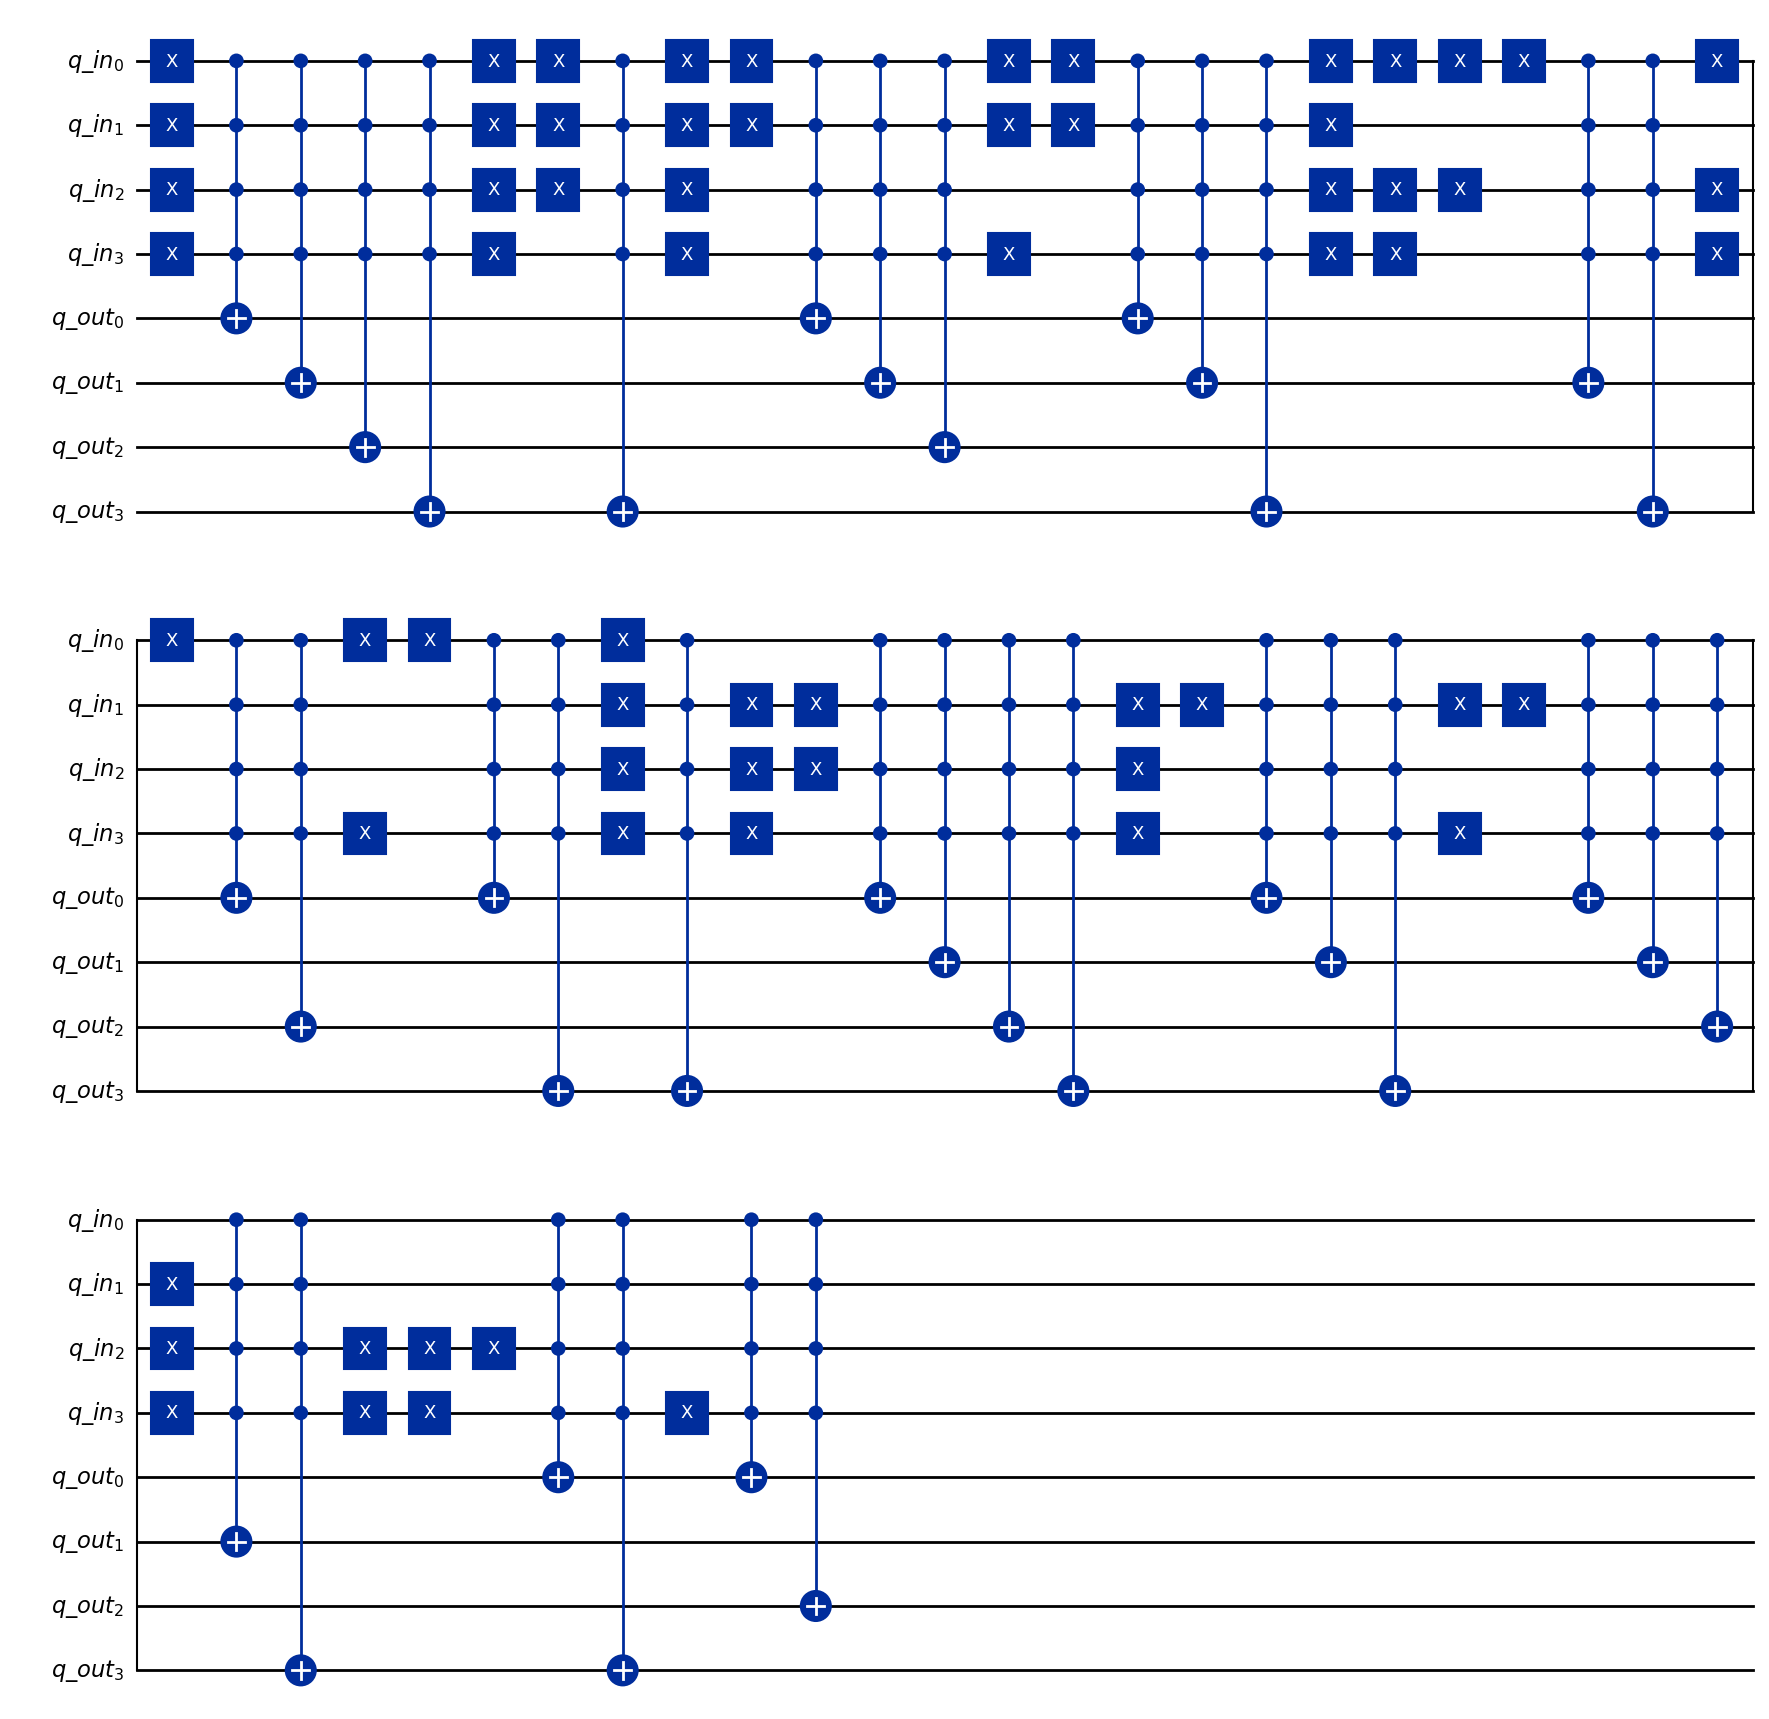
\includegraphics[width=0.5\linewidth]{Images/simon_oracleex2.png}
    \caption{Simons algorithm oracle}
    \label{fig:simon_oralce}
\end{figure}
Similarly, we can create the oracle for any such secret string.

The circuit, along with the corresponding oracle can be implemented using the following code
\begin{lstlisting}[language=Python]
qc = simon_circuit(build_oracle(f))
qc.draw(output="mpl")
\end{lstlisting}
The circuit implementing the function, is shown in Figure~\ref{fig:simon}.

\begin{figure}[ht]
    \centering
    \includegraphics[width=\linewidth]{Images/simon.png}
    \caption{Simons Algorithm circuit}
    \label{fig:simon_circ}
\end{figure}

Note that the oracle shown implements the function $f(x) = s \cdot x$ with some secret string $s$.

\item \textbf{Step 2: Optimize problems for quantum execution}
\begin{lstlisting}[language=Python]
target=backend.target
pm = generate_preset_pass_manager(backend=backend, optimization_level=3)

circuit_isa_qc=pm.run(qc)
circuit_isa_qc.draw(output="mpl",idle_wires=False,style="iqp")
\end{lstlisting}


\begin{figure}[ht]
    \centering
    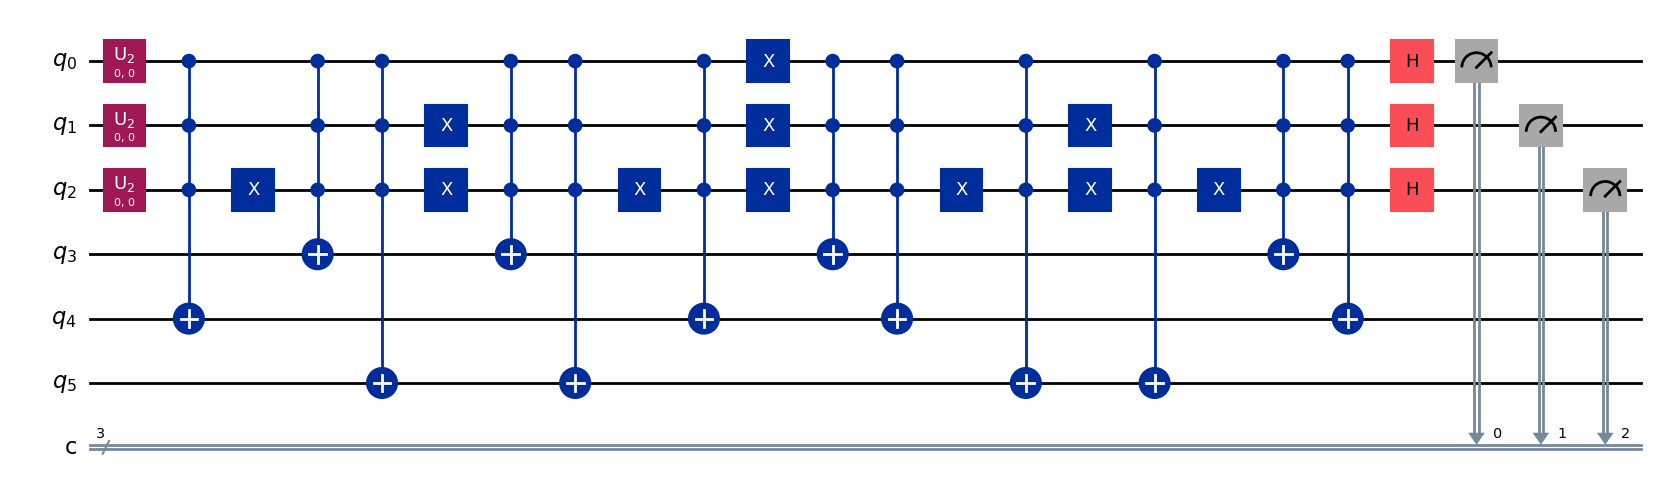
\includegraphics[width=\linewidth]{Images/simon_opt.png}
    \caption{Simon algorithm transpiled circuit}
    \label{fig:simon_opt}
\end{figure}

The optimized circuit shown in Figure~\ref{fig:simon_opt} is the one that will actually be executed on a quantum computer.

\item \textbf{Step 3: Execute using Qiskit Primitives} \\
We now run the circuit and sample the measurements on the first $n$ qubit. For execution, we use the \texttt{Sampler} runtime primitive.

    
\begin{lstlisting}[language=Python]
sampler=Sampler(mode=backend)
sampler.options.default_shots=10_000
result = sampler.run([circuit_isa_qc]).result()
dist = result[0].data.c.get_counts()
\end{lstlisting}
    
The output of the above code will be a distribution of measurements equal to the size of the secret string.

\item \textbf{Step 4: Post-process results} \\
Now we plot a histogram of the measurements in classical format.

    
\begin{lstlisting}[language=Python]
from qiskit.visualization import plot_histogram
plot_histogram(dist)
\end{lstlisting}
    
The output of the above code will be a histogram showing the distribution of measurements.

The following output is produced upon running the code on \texttt{ibm\_brisbane}, as shown in Figure~\ref{fig:simon_hist}. The histogram plot is based on 10,000 shots, and the results clearly align with expectations. Minor deviations arise due to the inherent noise in quantum hardware and the probabilistic nature of quantum measurements.

\begin{figure}[ht]
    \centering
    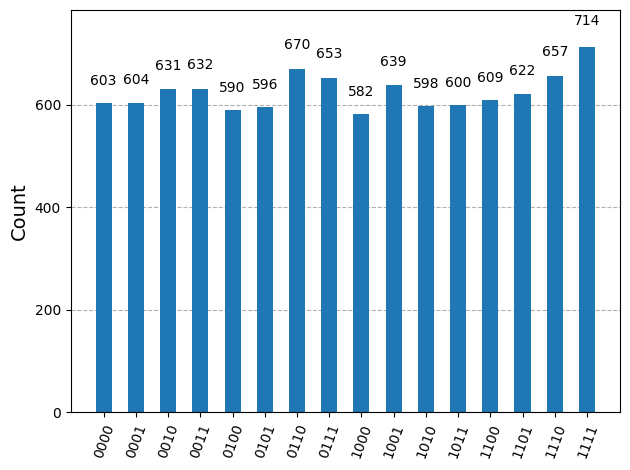
\includegraphics[width=\linewidth]{Images/simon_hist.png}
    \caption{Histogram of measurements}
    \label{fig:simon_hist}
\end{figure}

As seen in Figure~\ref{fig:simon_hist}, the measurement outcome with the maximum occurrence are the strings $1011$. Due to the Little Endian convention, this corresponds to the strings $s = 1101$ in classical format. This can be done using the following code:
\begin{lstlisting}[language=Python]
# Revese the bit order in the keys
dist_reversed = {key[::-1]: value for key, value in dist.items()}
#Pick the top 4 keys
top_keys = sorted(dist_reversed, key=dist_reversed.get, reverse=True)[:4]
print("Top 4 keys:", top_keys)
\end{lstlisting}
Now we do classical post-processing i.e.e form a matrix and solve for its null space in mod 2 arithmetic. This can be done using the following code:
\begin{lstlisting}[language=Python]
# Step 1: Create binary matrix from strings
matrix = np.array([list(map(int, key)) for key in top_keys])
print("Matrix from top keys:")
print(matrix)

# Step 2: Convert to sympy Matrix and reduce mod 2
A = Matrix(matrix)
A_mod2 = A.applyfunc(lambda x: x % 2)

# Step 3: Compute nullspace over GF(2)
nullspace = A_mod2.nullspace(iszerofunc=lambda x: x % 2 == 0)

# Step 4: Convert each sympy vector to numpy array with mod 2
nullspace_numpy = [np.array(vec.applyfunc(lambda x: x % 2)).astype(int).flatten() for vec in nullspace]

# Output
print("\nNullspace basis vectors over GF(2) (as numpy arrays):")
for vec in nullspace_numpy:
    print(vec)

# Convert each nullspace basis vector to a bit string
bit_strings = [''.join(map(str, vec)) for vec in nullspace_numpy]
string = ''.join(bit_strings)
print("The string is s:",string)
\end{lstlisting}
This confirms that the string is $s = 1101$, as expected. You are encouraged to try this with different strings and functions.
\end{enumerate}


